\documentclass[journal]{new-aiaa}
\usepackage[utf8]{inputenc}

\usepackage{graphicx}
\usepackage{subcaption}
\usepackage{amsmath}
\usepackage[version=4]{mhchem}
\usepackage{siunitx}
\usepackage{float}
\usepackage{array}
\usepackage[export]{adjustbox}
\usepackage{longtable, tabularx}
\usepackage{tabulary}
\usepackage{graphicx,color}
\usepackage{atbegshi,picture}
\usepackage{color, colortbl}
\graphicspath{./figures/}
\setlength\LTleft{0pt} 

\title{A Study On The Efficacy of Using Eigenfaces In Image Classification}
        
\author{Jacob T. Cassady\footnote{Graduate Student, Robotics and Autonomous Systems}, Dimitri Medina\footnote{Graduate Student, Mechanical Engineering}}
\affil{Johns Hopkins University, Whiting School of Engineering, Baltimore, MD, 21206}

\begin{document}

\maketitle
\begin{abstract}
The increased use of image classification in technology today has incited a rise in research and development for new approaches in facial detection and identification models. 
Two common problems in image classification are storing large datasets and model training costs.
One approach to achieving dimensionality reduction while maintaining performance is Principal Component Analysis where a subset of eigenvectors, also known in the domain of facial detection as ``eigenfaces'', are used to represent the data in a lower dimensionality space.
This paper presents an image classification model based on eigenfaces and support vector machines using the Amsterdam Dynamic Facial Expression Set (ADFES) dataset. 
Implementation of an image classification model is described, and performance analysis of the model is presented with a focus on the efficacy of using eigenfaces when training the model.
\end{abstract}

\section{Nomenclature}\label{sec:Nomenclature}

{\renewcommand\arraystretch{1.0}
\noindent\begin{longtable*}{@{}l @{\quad=\quad} l@{}}
$ADFES$  &    Amsterdam Dynamic Facial Expression Set \\
$AICE$   &    Amsterdam Interdisciplinary Centre for Emotion \\
$PCA$    &    Principal Component Analysis \\
$SVM$    &    Support Vector Machine \\
\end{longtable*}}

\section{Introduction}\label{sec:Introduction}
Image classification has become an innovation of interest in recent years due to the parallel advances in machine learning techniques, digital camera technology, and other similar computational fields of science. 
From security monitoring to access control, image classification has become an important tool in many diverse disciplines. 
Two common problems in image classification are storing large datasets and model training costs.

One approach to achieving dimensionality reduction while maintaining a representation of the data is Principal Component Analysis (PCA) \cite{abdi2010principal}.
In the field of facial recognition, PCA can remove the reliance on the isolation of features such as eyes and ears, and instead takes a mathematical approach to defining and characterizing face images. 
PCA uses a subset of eigenvectors, also known in facial recognition as ``eigenfaces'', to represent the data in a lower dimensionality space.
If a certain characteristic is prominent in a collection of images, the eigenface corresponding to the characteristic has a larger eigenvalue and represents a higher explained variance of the dataset \cite{turk1991face}. 
After utilizing PCA, eigenvectors of lesser importance can be removed to reach a desired level of dimensionality reduction with the trade-off of reduced explained variance of the initial dataset.

SVMs are supervised learning algorithms designed to find the optimal hyperplane that maximizes the margin between the closest data points of opposite classes \cite{708428}.
SVMs suffer high computational costs when the number of features is large.
Using eigenvectors calculated with PCA has been shown to work well with Support Vector Machines (SVMs) for classification in a variety of domains \cite{mangasarian2005multisurface}\cite{alvarez2009alzheimer}\cite{melivsek2008support}.

This paper focuses on analyzing the efficacy of using eigenfaces when performing image classification of the Amsterdam Dynamic Facial Expression Set (ADFES) dataset using SVMs.
Section \ref{sec:Dataset} provides a description of the ADFES dataset.
Section \ref{sec:Model} introduces the model used for image classification including the mathematics of eigenfaces and SVMs.
Section \ref{sec:Implementation} describes the implementation of a classification model using eigenfaces and SVMs with the Python programming language.
Section \ref{sec:Analysis} presents analysis of the classification model including the efficacy of using eigenfaces in image classification.
This paper concludes with a discussion of the results and future work in sections \ref{sec:Discussion} and \ref{sec:Future Work} respectively.

\section{Amsterdam Dynamic Facial Expression Set}\label{sec:Dataset}
The ADFES dataset was developed by the University of Amsterdam's Amsterdam Interdisciplinary Centre for Emotion (AICE) \cite{adfes}.
The ADFES dataset includes expressions displayed by 22 models from Northern-European and Mediterranean locations.
There are ten emotions included in ADFES dataset: anger, contempt, disgust, embarrassment, fear, joy, neutral, pride, sadness, and surprise.
The ADFES dataset includes both videos and still images.
Each media is labeled with a gender: male or female.
This paper will utilize the 217 still images from the ADFES dataset only.
Figure \ref{fig:ExampleImage} includes an example of a still image from the ADFES dataset.
Table \ref{table:Target Class Distributions} shows the number of classes per target in the dataset and the images per class.
Each image has a width of 720, a height of 576, and three 8-bit color channels: red, green, and blue.

\begin{figure}[H]
  \centering
  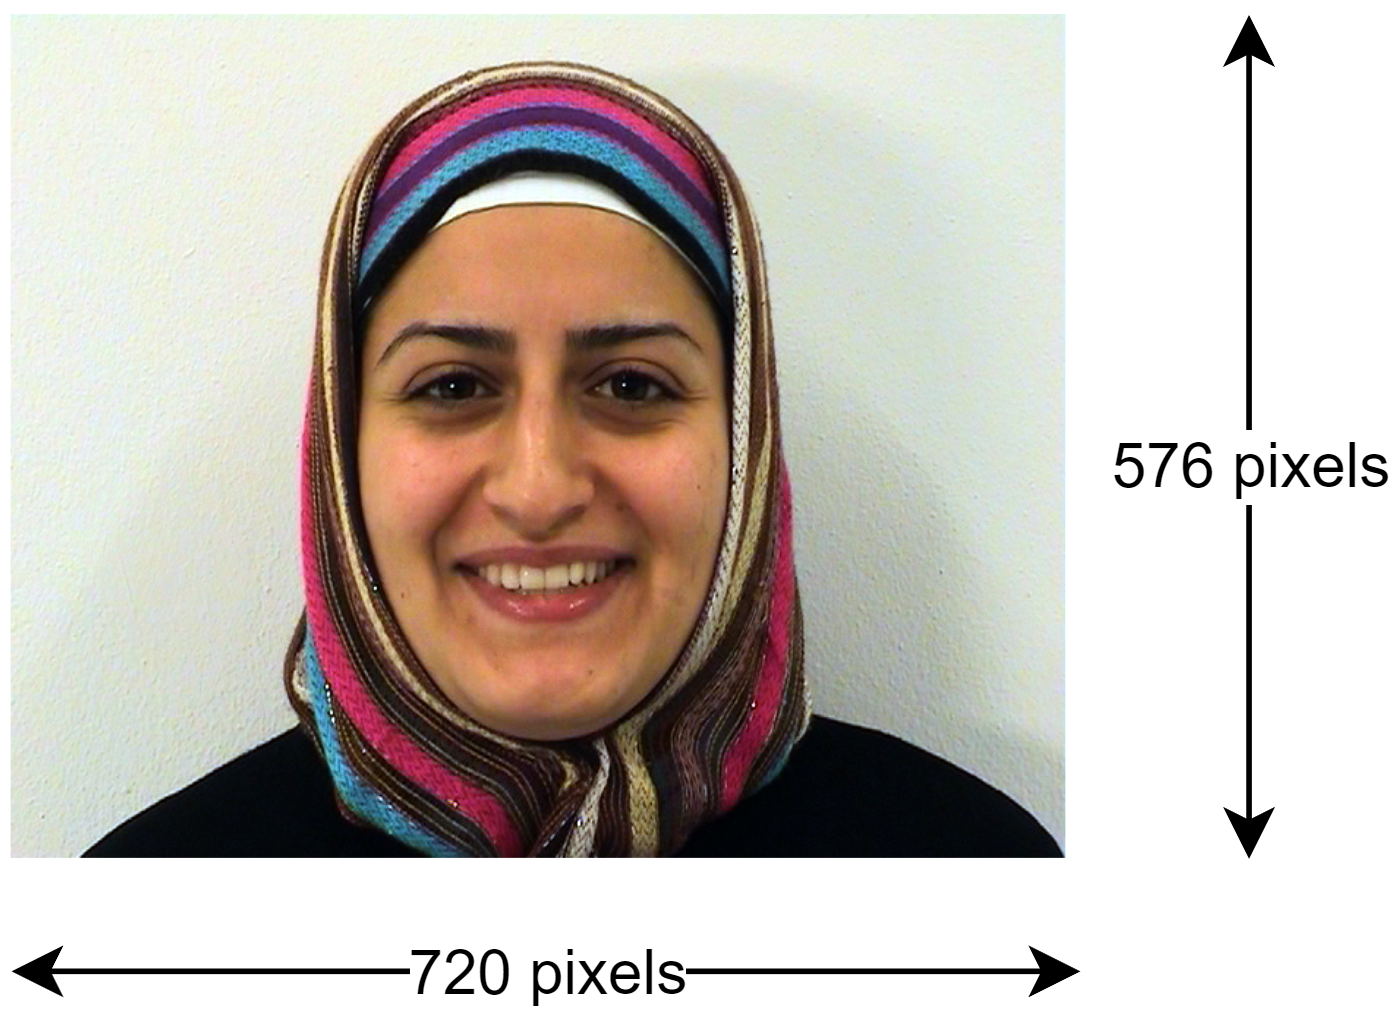
\includegraphics[width=.3\textwidth]{figures/Image Example.PNG}
  \caption{ADFES Example Image with targets: Mediterranean, Female and Joy}
  \label{fig:ExampleImage}
\end{figure}

\begin{table}[H]
  \centering
  \begin{tabular}{|| c | c | c ||} 
          \hline
          Target               & Class Count & Images Per Class \\ [0.5ex] 
          \hline\hline
          Geographic Tag       & 2 & \{Northern European: 120, Mediterranean: 97\} \\ [0.5ex] 
          \hline
          Gender Tag           & 2 & \{Male: $\approx120$, Female: $\approx100$\} \\ [0.5ex] 
          \hline
          Model Identification & 22 & $\approx 10$ \\ [0.5ex] 
          \hline
          Emotion              & 10 & $\approx 22$ \\ [0.5ex] 
          \hline
  \end{tabular}
  \caption{Target Class Distributions}
  \label{table:Target Class Distributions}
\end{table}

\section{Model}\label{sec:Model}
Image classification will be accomplished using eigenfaces and SVMs.
Calculation of eigenfaces, or more generally eigenvectors, will be calculated using Principal Component Analysis (PCA).
Section \ref{sec:Model:Features and Targets} describes the shapes of the feature and target matrices before the eigenface dimensionality reduction described in Section \ref{sec:Model:Eigenfaces}.
Section \ref{sec:Model:SVM} describes the mathematics of a SVM.

\subsection{Features and Targets}\label{sec:Model:Features and Targets}
Each image $I$ of the dataset follows the representation shown in equation \ref{eqn:image}.
As previously mentioned, each image begins with shape ($576\ height$, $720\ width$, $3\ color\ channels$).

\begin{equation}\label{eqn:image}
  I(i)=\begin{bmatrix} (r_{(0,0)}, g_{(0,0)}, b_{(0,0)}) & (r_{(0,1)}, g_{(0,1)}, b_{(0,1)}) & \dots & (r_{(0,719)}, g_{(0,719)}, b_{(0,719)}) \\
    (r_{(1,0)}, g_{(1,0)}, b_{(1,0)}) & (r_{(1,1)}, g_{(1,1)}, b_{(1,1)}) & \dots & (r_{(1,719)}, g_{(1,719)}, b_{(1,719)}) \\
    \dots & \dots & \dots & \dots \\
    (r_{(575,0)}, g_{(575,0)}, b_{(575,0)}) & (r_{(575,1)}, g_{(575,1)}, b_{(575,0)}) & \dots & (r_{(575,719)}, g_{(575,719)}, b_{(575,719)}) \\
  \end{bmatrix}
\end{equation}

The images are first flattened as shown in equation \ref{eqn:flattened-image}.

\begin{equation}\label{eqn:flattened-image}
  I(i)_{flat}=
  \begin{bmatrix} r_{(0,0)} & g_{(0,0)} & b_{(0,0)} & \dots & r_{(0,719)} & g_{(0,719)} & b_{(0,719)} \dots r_{(575,719)} & g_{(575,719)} & b_{(575,719)}
  \end{bmatrix}
\end{equation}

The flattened images are then stacked on top of each other to create a matrix of features as shown in equation \ref{eqn:features}.

\begin{equation}\label{eqn:features}
  features=\begin{bmatrix} I(0)_{flat} \\ I(1)_{flat} \\ \dots \\ I(216)_{flat} \end{bmatrix},\ targets=\begin{bmatrix} T(0) \\ T(1) \\ \dots \\ T(216) \end{bmatrix}
\end{equation}

The final feature matrix will be of shape (217, 1,244,160).
The target matrix is created by retrieving the column matching the target data.
If the target data is in the form of a label, each string is encoded into an integer matching the class.
In the example of gender, males would be encoded to 1 and female encoded to 2.
The final target matrix will be of shape (217, 1).

Before feeding into the model for training, the data was randomly shuffled and then split into training and validation sets.
With an 80-20 training and validation split, 172 images and associated targets were placed in the training set and 44 images and associated targets were placed in test set.
The training features and validation features were of shapes (172, 1,244,160) and (44, 1,244,160) respectively.
The training targets and validation targets were of shapes (172, 1) and (44, 1) respectively.

\subsection{Principal Component Analysis}\label{sec:Model:Eigenfaces}
PCA can be used to achieve dimensionality reduction while maintaining a representation of the data \cite{abdi2010principal}.
PCA uses a subset of eigenvectors, also known in facial recognition as ``eigenfaces'', to represent the data in a lower dimensionality space.
Eigenvectors will each have an associated eigenvalue which is a scalar and is a measure of the eigenvector prominence in the dataset. 

To calculate the eigenfaces, processing of the face images and the calculation of the covariance matrix must be done.
Each face image $I(i)$ will be represented as a vector $\varGamma_n$. 
The vectors $\varGamma_n$ will then be used to calculate the average matrix $\Psi$ of each component as shown in equation \ref{eqn:Average Matrix}.

\begin{equation}\label{eqn:Average Matrix}
  \Psi = \frac{1}{N} \sum_{n=1}^{M} \varGamma_n  
\end{equation}

The resulting matrix will then be subtracted from each face image and stored in the variable $\Phi_n$ as shown in equation \ref{eqn:Distance To Mean}.
$\Phi_n$is used to calculate the covariance matrix $C$ as shown in equation \ref{eqn:Covariance Matrix}.

\begin{equation}\label{eqn:Distance To Mean}
  \Phi_n = \varGamma_n - \Psi
\end{equation}

\begin{equation}\label{eqn:Covariance Matrix}
  C = \frac{1}{M} \sum_{n=1}^{M} \Phi_n \Phi_n^T = A A^T,\ \text{where}\ A = [\Phi_1, \Phi_2, \dots, \Phi_M]
\end{equation}

The covariance matrix has the eigenfaces $u_i$ and their respective eigenvalues $v_i$ as shown in equation \ref{eqn:cvu}, where $u_i$ is solved with equation \ref{eqn:ui}.
Finally, it is important to normalize $u_i$ such that $||u_i||=1$.
 
\begin{equation}\label{eqn:cvu}
  A^T A v_i = u_i v_i
\end{equation}

\begin{equation}\label{eqn:ui}
  u_i = \sum_{k=1}^{M} v_{lk} \Phi_k,\ \text{where}\ l = 1, 2, \dots, M
\end{equation}

The training features and validation features after the eigenface transform were of shapes (172, $E_{count}$) and (44, $E_{count}$) respectively where $E_{count}$ is the number of components (eigenvectors or eigenfaces) from PCA retained.
As described in Section \ref{sec:Analysis:Classification Analysis}, different values of $E_{count}$ were chosen for different targets.
A higher $E_{count}$ value means lower dimensionality reduction and higher explained variance of the input feature space. 

\subsection{Support Vector Machine}\label{sec:Model:SVM}
SVMs are supervised learning algorithms designed to find the optimal hyperplane that maximizes the margin between the closest data points of opposite classes \cite{708428}.
Multiclass classification can be achieved using a One-to-One or a One-to-Rest approach.
The closest datapoints are also called ``support vectors''.
SVM classifiers are based on the class of hyperplanes shown in equation \ref{eqn:hyperplane class}.

\begin{equation}\label{eqn:hyperplane class}
  (w \bullet x) + b = 0,\\ w \in \Re^N,\ b\in \Re
\end{equation}

The optimal hyperplane can be found by solving a constrained optimization problem whose solution $w$ has an expansion shown in equation \ref{eqn:optimization problem} where $x_i$ is one training example.
Solutions to SVMs can be generated using quadratic programming.

\begin{equation}\label{eqn:optimization problem}
  w=\sum_{i = 1}^{N} v_i x_i 
\end{equation}

SVMs perform a nonlinear separation from the input space into a higher-dimensional ``feature space'' $F$ as shown in equation \ref{eqn:feature space}.
The mapping performed by the SVM is called the kernel function $K(x, y)$.
This paper will focus on the linear kernel defined by equation \ref{eqn:linear kernel}

\begin{equation}\label{eqn:feature space}
  \Phi : \Re^N \rightarrow F
\end{equation}

\begin{equation}\label{eqn:linear kernel}
  K(x, y) = \Phi (x) \bullet \Phi (y)
\end{equation}

The decision function for the SVM is shown in equation \ref{eqn:SVM decision function} where $v_i$ are the parameters calculated using quadratic programming.

\begin{equation}\label{eqn:SVM decision function}
  f(x) = sign\left(\sum_{i = 1}^{l} v_i \bullet k(x, x_i) + b \right)
\end{equation}

\section{Implementation}\label{sec:Implementation}
To analyze the efficacy of eigenfaces for maintaining model performance while reducing the dimensionality of the data, the model described in section \ref{sec:Model} was implemented in Python 3.8.
Table \ref{table:3rd Party Libraries Used} lists the 3rd party libraries used in the implementation.
Section \ref{sec:Implementation:Data Preprocessing} describes the data preprocessing steps taken before feeding the data into the model.
Section \ref{sec:Implementation:Model Implementation} describes the implementation of the model.

\subsection{Data Preprocessing}\label{sec:Implementation:Data Preprocessing}
Images downloaded from the ADFES dataset were placed in two directories named after the geographic tag.
Files from the ADFES dataset included the regional model identification, emotion, and gender tag in the file name.
A global model identification value was calculated using equation \ref{eqn:GlobalModelID} where $ID_{Max}$ is the largest regional model id in the dataset, $G$ is an enumeration dependent on the geographic tag on the image, and $S$ is an enumeration dependent on the gender tag on the image.
A python script was written to place image data into a pandas \cite{pandas} DataFrame with rows representing an image with associated metadata and columns representing the geographic tag, model identification, emotion, gender tag, and pixel values.
After preprocessing the data, the pandas data structure was stored using a Python pickle file.

\begin{equation}\label{eqn:GlobalModelID}
  ModelID_{Global}= ModelID_{Regional} + (ID_{Max}+1)(G + 2 S)
\end{equation}

To format the data for usage by the model, pixel data was flattened for each image into a single row as shown in Equation \ref{eqn:flattened-image}.
Each row of image data was then stacked on top of each other to form a matrix of features of shape (217, 1,244,160).
The training column was extracted from the pandas DataFrame and formatted as a NumPy array of shape (217,1).
The sci-kit learn \cite{scikit-learn} LabelEncoder preprocessing class was used to convert string labels into integer values.
Data was then randomly shuffled and split into train and validation sets using sci-kit learn's train\_test\_split method.

\subsection{Model Implementation}\label{sec:Implementation:Model Implementation}
To calculate the eigenvalues of the data, sci-kit learn's Principal Component Analys (PCA) class was used.
The singular value decomposition solver was set to ``randomized'' - meaning it calculated the eigenfaces using the method described by Halko et al. \cite{halko2011finding}.
The sci-kit learn SVC class was used for support vector machine classification.
The regularization parameter $C=3$ and a linear kernel were used.

\section{Analysis}\label{sec:Analysis}
The primary benefit of using eigenfaces is dimensionality reduction, therefore the analysis section focuses on the trade off between using eigenfaces to reduce datasize and maintaining model performance.
Section \ref{sec:Analysis:Eigenface Analysis} provides analysis of Eigenface Count's ($E_{count}$) effect on model training performance.
Section \ref{sec:Analysis:Classification Analysis} presents the performance of the best model for each target in the ADFES dataset with the largest amount of dimensionality reduction.

\subsection{Eigenface Analysis}\label{sec:Analysis:Eigenface Analysis}
As previously stated, the number of eigenfaces retained from PCA determines the amount of explained variance represented by the eigenface features when compared to the input features.
Figure \ref{fig:EEA0} shows the performance of the SVM on each target with $E_{count}$ values ranging from [2, 10].
This analysis was performed 5 times for each data point.
The left Y-axis represents the accuracies of the models.
The center blue dots represent the average model accuracy over the five tests while the blue lines represent the standard deviations of the accuracies.
The purple lines represent the amount of explained variance in the eigenface features used in training the model.
Figure \ref{fig:EEA1} shows the performance of the SVM on each target with $E_{count}$ values ranging from [10, 125].

\begin{figure}[H]
  \centering
  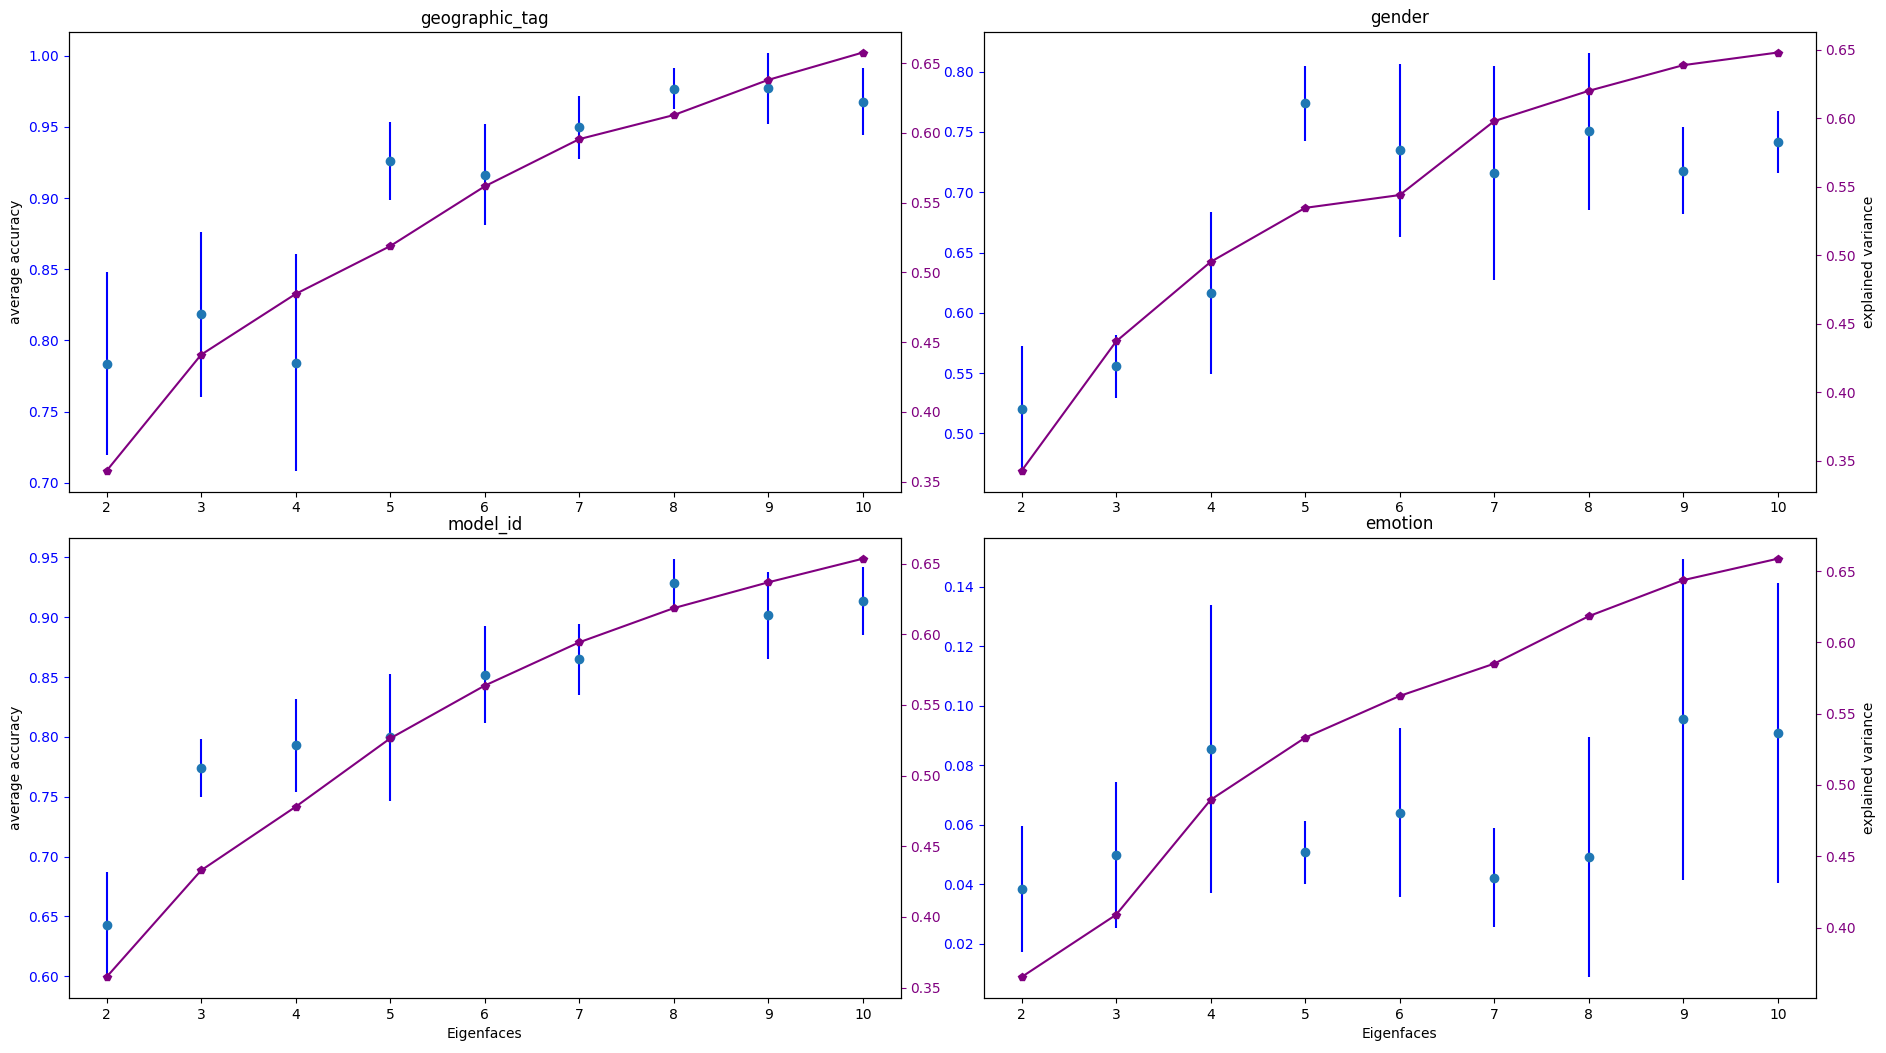
\includegraphics[width=.9\textwidth]{figures/eigenface_analysis_2_10.png}
  \caption{Eigenface Efficacy Analysis (2-10 eigenfaces). The x-axis of each plot is the number of eigenfaces used in the training. The left y-axis for each plot is the average weighted accuracy over 5 tests. The right y-axis for each plot is the total explained variance of the eigenfaces used in the training.}
  \label{fig:EEA0}
\end{figure}

Analyzing the eigenfaces directly can provide valuable insight into the dataset.
As shown in Figure \ref{fig:EEA0}, the top 9 eigenfaces shown in Figure \ref{fig:Top 9} represent more than 65\% of the explained variance in the input features.

\begin{figure}[H]
  \centering
  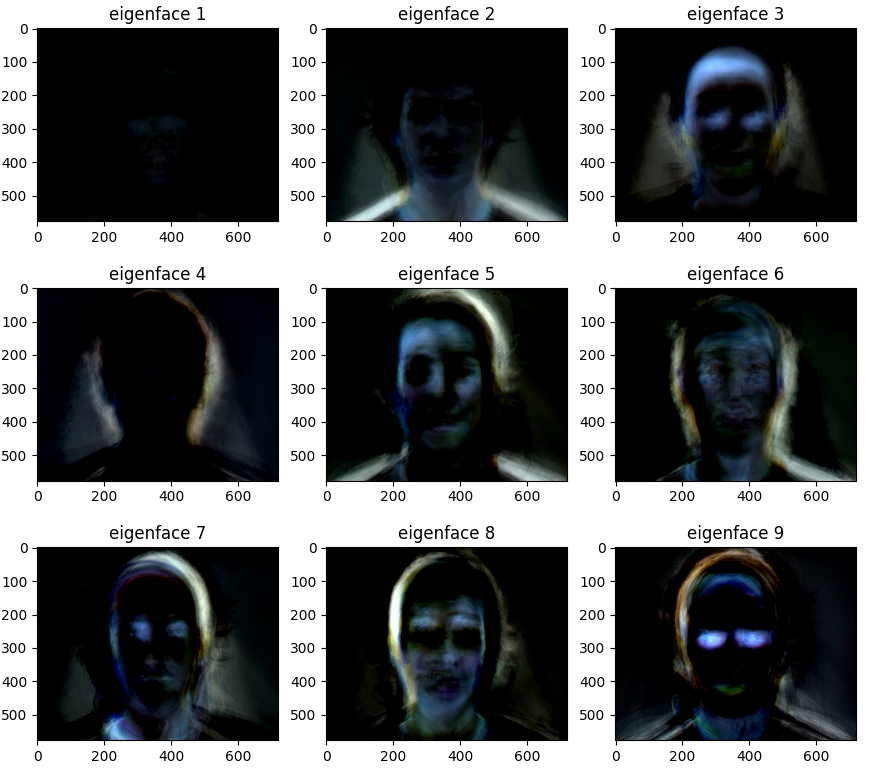
\includegraphics[width=.8\textwidth]{figures/top_9_eigenfaces.png}
  \caption{Top 9 Eigenfaces}
  \label{fig:Top 9}
\end{figure}

\subsection{Classification Analysis}\label{sec:Analysis:Classification Analysis}
Before performing PCA, features and targets were randomly shuffled.
80\% of the data or 172 images and associated targets were placed in training set.
20\% of the data or 44 images and associated targets were placed in test set.
Models were trained to classify each target in the dataset: geographic tag, gender tag, model identification, and emotion.
Each model was trained for a maximum of 5 times and the best outcome was retained.
The $F_1$ score, also known as the harmonic mean of the precision and recall, is the performance metric chosen for comparing models.
Equation \ref{eqn:$F_1$} for $F_1$ score can be found below.

\begin{equation}\label{eqn:$F_1$}
  F_1=2\frac{precision \bullet  recall}{precision + recall}
\end{equation}

Table \ref{table:Best Model Performances} presents the performance of the model on each target.
Eigenface count ($E_{count}$) represents the number of eigenfaces with the highest explained variances retained after performing PCA.
The explained variance column represents the sum of explained variances of all eigenfaces used in the target's model.
$E_{count}$ values were chosen analytically from inspecting Figure \ref{fig:EEA1} and selecting the smallest $E_{count}$ with the best performance.
Data size reduction was calculated with the formula shown in equation \ref{eqn:data size reduction}.

\begin{equation}\label{eqn:data size reduction}
  \texttt{Data Size Reduction} = \frac{size(EigenfaceFeatures) - size(Features)}{size(Features)}\bullet 100\%
\end{equation}

\begin{table}[H]
  \centering
  \begin{tabular}{|| c | c | c | c | c ||} 
          \hline
          Target               & $E_{count}$ & Explained Variance & Data Size Reduction & Best $F_1$ Score \\ [0.5ex] 
          \hline\hline
          Geographic Tag       & 50 & $\approx$ 87\% & -99.9960\% & 1.00 \\ [0.5ex] 
          \hline
          Gender Tag           & 65 & $\approx$ 90\% & -99.9948\% & 1.00 \\ [0.5ex] 
          \hline
          Model Identification & 50 & $\approx$ 87\% & -99.9960\% & 1.00 \\ [0.5ex] 
          \hline
          Emotion              & 75 & $\approx$ 92\% & -99.9940\% & 0.293 \\ [0.5ex] 
          \hline
  \end{tabular}
  \caption{Best Model Performances}
  \label{table:Best Model Performances}
\end{table}

Confusion matrices were also generated to provide insight into the model's performance on the validation set per class of the target.
The confusion matrices for geographic tag, gender, model identification, and emotion can be found in Figures \ref{fig:Geographic Confusion Matrices}, \ref{fig:Gender Confusion Matrices}, \ref{fig:Model Identification Confusion Matrices}, and \ref{fig:Emotion Confusion Matrices} respectively.

\begin{figure}[H]
  \centering
  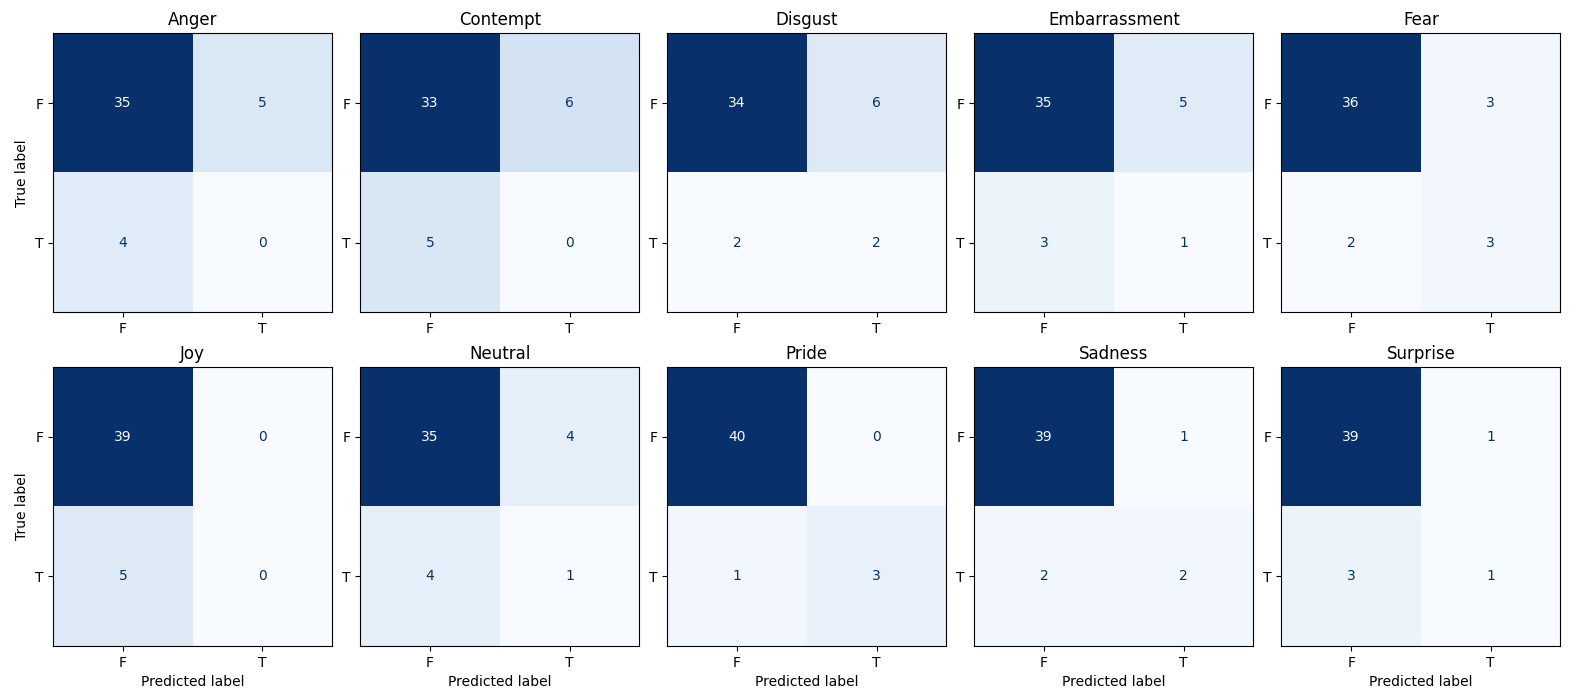
\includegraphics[width=\textwidth]{figures/emotion_tag_cm.png}
  \caption{Emotion Confusion Matrices}
  \label{fig:Emotion Confusion Matrices}
\end{figure}

\section{Discussion}\label{sec:Discussion}
Eigenfaces retain high classification accuracy while achieving dimensionality reduction.
Figure \ref{fig:EEA0} shows the performance of the model on each target with 2-10 eigenfaces and Figure \ref{fig:EEA1} shows the performance of the model on each target with 10-125 eigenfaces.
With only the top nine eigenfaces, shown in Figure \ref{fig:Top 9}, the model was able to achieve an $F_1$ Score of more than 90\% on geographic tag and model identification targets.
Table \ref{table:Best Model Performances} shows a perfect $F_1$ Score was achieved on 3 of the 4 targets with a data size reduction of more than 99.99\% from using eigenfaces.

High classification accuracy was achieved on all targets except emotion. 
Table \ref{table:Best Model Performances} shows the best performance of the support vector machine classifier on each target.
The confusion matrix for emotion shown in Figure \ref{fig:Emotion Confusion Matrices} provides insight into the model's performance issues with emotion classification.
The model is over-classifying for anger, contempt, disgust, embarrassment, and neutral while under-classifying for emotions like joy, pride, sadness, and surprise.
The poor performance of the model on classifying emotion is possibly due to the relatively low amount of data per emotion class in the ADFES still images.

The ADFES dataset was chosen to test the benefit of eigenfaces because of the low development cost for preprocessing the data.
Additionally, the ADFES dataset includes still images that are centered on the model's face.
The consistent positioning provides good insight into what an eigenface, and more generally what an eigenvector, represents in the context of PCA.
Because still, well-formatted, images were used to train and validate the model described in this paper is unlikely to perform well in computer vision systems that have dynamic angles on their subject.

\section{Future Work}\label{sec:Future Work}
The choice to focus on still images was secondary to schedule.
The model's performance on classifying emotions could be greatly improved by increasing the number of images per emotion.
Images could be extracted from the video data in the ADFES dataset.
Images could also be generated using data augmentation methods \cite{maharana2022review}.
The model would also benefit from diverse camera angles.

The ADFES dataset included images with participants from two geographic tags: Northern European and Mediterranean.
It is important to understand the populations represented in a dataset to understand what populations the model has been validated on.
For consistent performance across larger populations, there needs to be more diversity in the training and validation sets \cite{zou2018ai}.

\section*{Appendix}\label{sec:Appendix}

\begin{figure}[H]
  \centering
  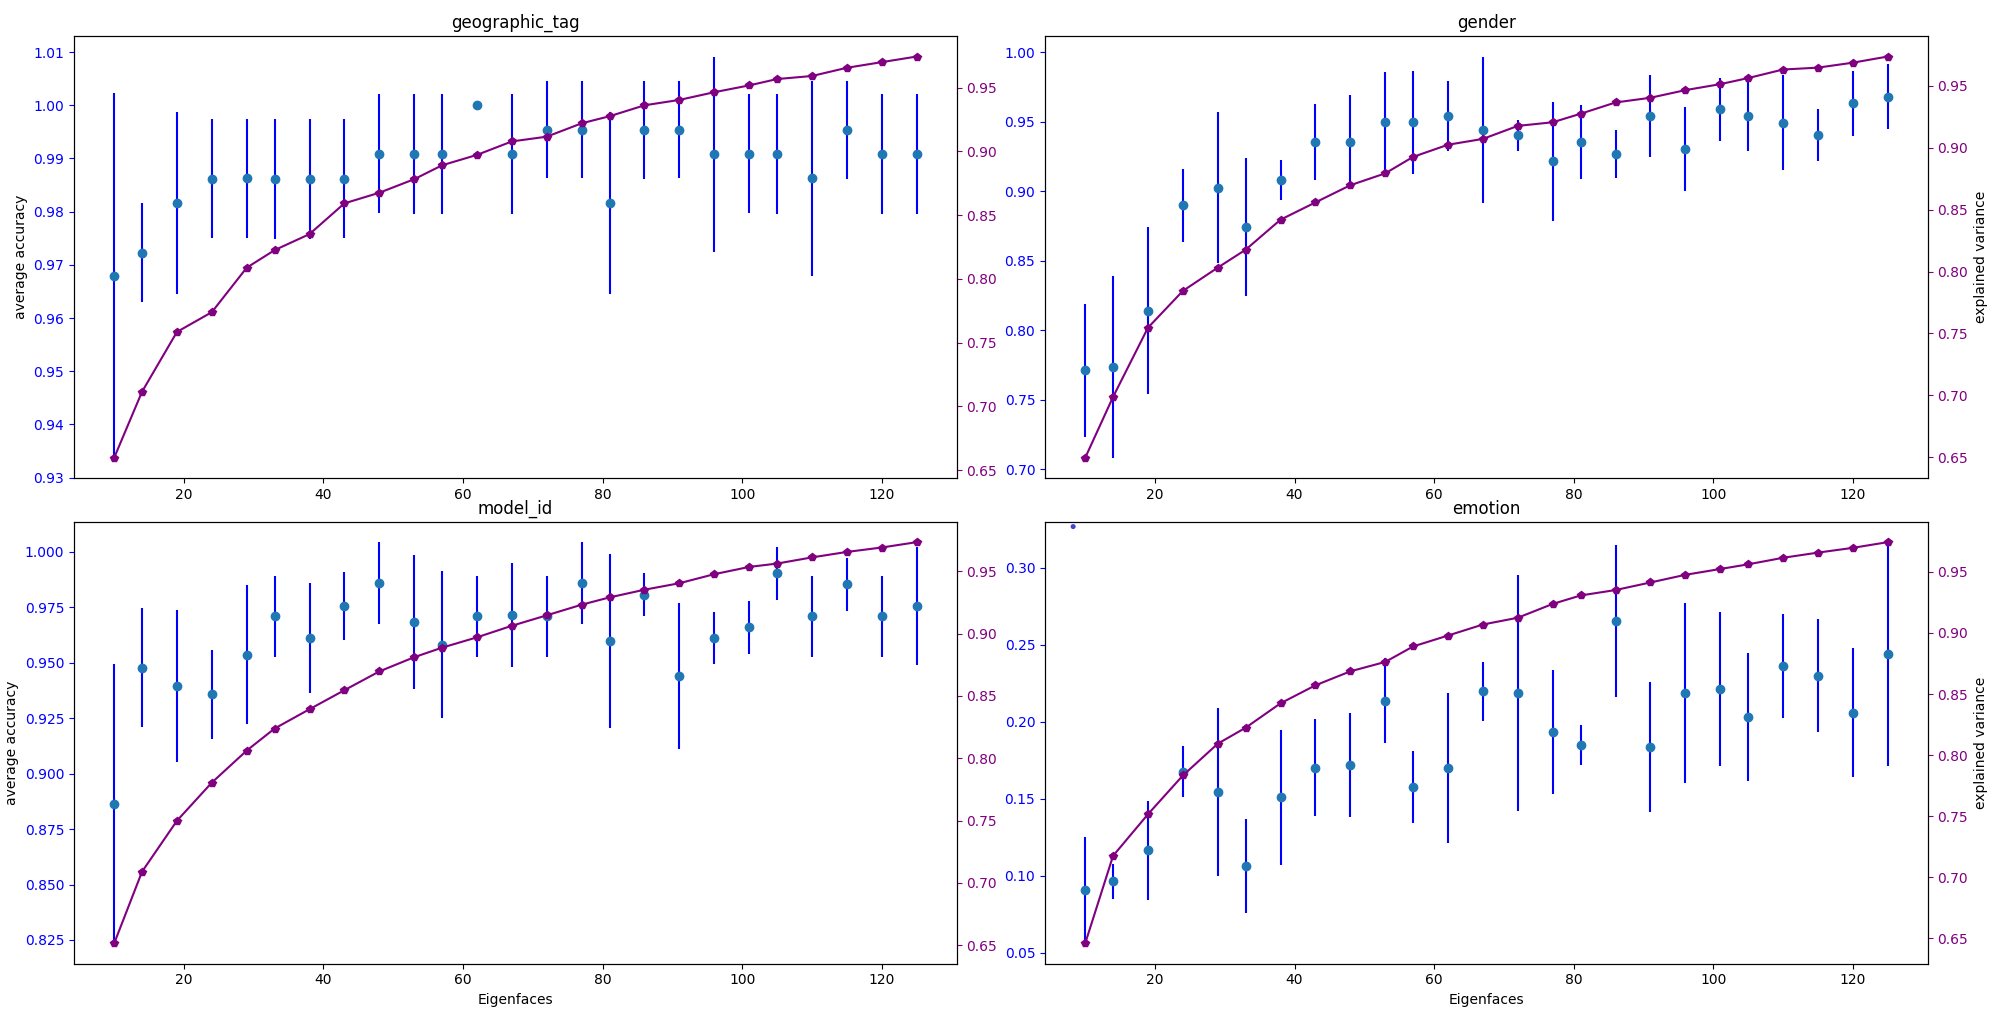
\includegraphics[width=\textwidth]{figures/eigenface_analysis_10_125.png}
  \caption{Eigenface Efficacy Analysis (10-125 eigenfaces). The x-axis of each plot is the number of eigenfaces used in the training. The left y-axis for each plot is the average weighted accuracy over 5 tests. The right y-axis for each plot is the total explained variance of the eigenfaces used in the training.}
  \label{fig:EEA1}
\end{figure}

\begin{figure}[H]
  \centering
  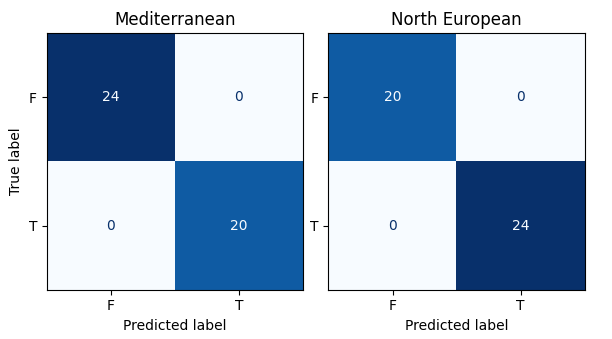
\includegraphics[width=.7\textwidth]{figures/geographic_tag_cm.png}
  \caption{Geographic Tag Confusion Matrices}
  \label{fig:Geographic Confusion Matrices}
\end{figure}

\begin{figure}[H]
  \centering
  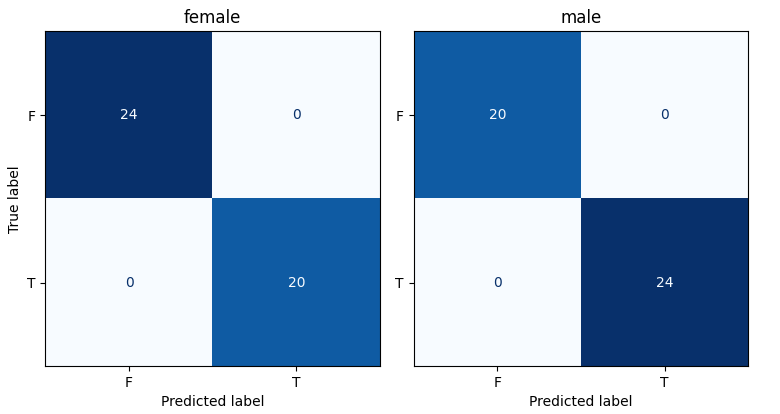
\includegraphics[width=.7\textwidth]{figures/gender_tag_cm.png}
  \caption{Gender Tag Confusion Matrices}
  \label{fig:Gender Confusion Matrices}
\end{figure}

\begin{figure}[H]
  \centering
  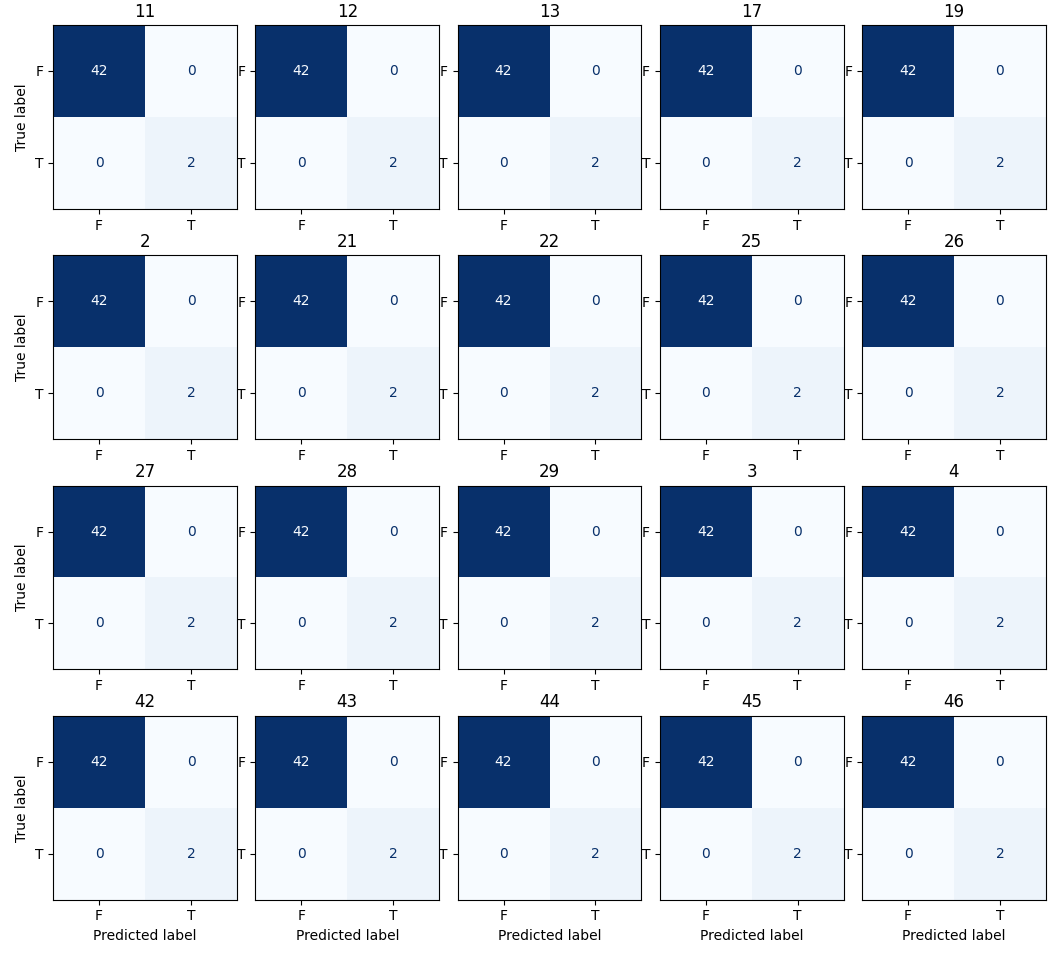
\includegraphics[width=.90\textwidth]{figures/model_id_tag_cm.png}
  \caption{Model Identification Confusion Matrices. Only 20 of the 22 model identities shown. The remaining 2 confusion matrices are the same as those shown.}
  \label{fig:Model Identification Confusion Matrices}
\end{figure}

\begin{table}[H]
  \centering
  \begin{tabular}{|| c | l | l ||} 
          \hline
          Name          & Description & Use \\ [0.5ex] 
          \hline\hline
          NumPy         & Comprehensive mathematical functions \cite{numpy} & Mathematical manipulations of data \\ [0.5ex] 
          \hline
          pandas        & Data analysis and manipulation tool \cite{pandas} & Store and filter data \\ [0.5ex] 
          \hline
          matplotlib    & Library for creating visualizations \cite{matplotlib} & Data inspection and performance plotting \\ [0.5ex] 
          \hline
          sci-kit learn & Tools for predictive data analysis \cite{scikit-learn} & PCA, train/test split, and SVM model \\ [0.5ex] 
          \hline
  \end{tabular}
  \caption{3rd Party Libraries Used}
  \label{table:3rd Party Libraries Used}
\end{table}

\section*{Acknowledgments}\label{sec:Acknowledgments}
This work was performed as a final paper for the Mathematical Methods for Engineers class at Johns Hopkins University taught by Professor George Nakos.

\bibliography{eigenfaces}

\end{document}